
\subsection{Model description}
The model is constructed as a rate network of two populations of neurons \textit{M} and \textit{P}, the former representing the memory trace of the \textit{K} available options (\textit{i.e.} the bandits), and the latter representing the value of the options under the current policy.
More formally, the model is described by a set of coupled ordinary differential equations (ODEs) that capture the decision-making process in two distinct neural spaces.
The first equation tracks the evolution of the neural activity $\textbf{u}$ of \textit{M}, while the second tracks the activity $\textbf{v}$ of the \textit{P}. The time constants $\tau$ are the same for both equations and are set to $\tau = 10$ ms.


\begin{equation}
\begin{aligned}
    \tau \dot{\textbf{u}}&= -\textbf{u} + \textbf{v} + \textbf{I}_{\text{ext}} \\
    \tau \dot{\textbf{v}}&= -\textbf{v} + \textbf{z} \odot\textbf{u}
\end{aligned}
\end{equation}

\noindent The external input $\textbf{I}_{\text{ext}}$ is a constant input that is used to set the initial conditions of the neural activity $\textbf{u}$.
The term $\textbf{z}$ is a vector that weights the contribution of the active options $\textbf{u}$ to the value representation $\textbf{v}$, and functionally it is the core of the policy adopted by the model.
In practice, $\textbf{z}$ defined as a function of the synaptic weights $\textbf{W}^{MP}$ from \textit{M} to \textit{P} as $\textbf{z} = \Phi_v(\textbf{W}^{MP})$. Importantly, the connections are not fully connected, but rather are simply one-to-one mapping between the corresponding neurons in each
population, such that the weight matrix $\textbf{W}^{MP}$ is simply a matrix $K\times 1$, namely a vector.
The function $\Phi_v$ is a chosen to be a sum of a generalized sigmoid and a Gaussian, whose contributions are weighted by a parameter $r$:

\begin{equation*}
    \Phi_v(x) = r\gamma_{1} \frac{1}{1 + e^{-\beta(x-\alpha)}} + (1-r)\gamma_{2} \exp\left(-\frac{(x-\mu)^2}{2\sigma^2}\right)
\end{equation*}

\noindent The motivation behind this choice is to express a function that possesses a bounded region (depending on $\mu,\,\sigma$) at a high/low peak (depeding on the value of $\gamma_{2}$), and a continuous transition to a constant value (depending on the steepness of the sigmoid $\beta$, shift
$\alpha$, and intensity $\gamma_{1}$).

% \hfill \break
\subsubsection{Option selection}
The decision-making process within a single round is structured in two distinct phases. Initially, the model receives a constant external input targeting all neurons in the memory population \textit{M} equally.
During this phase, $I_{\text{ext}}$ works as an equilibrium value while the reciprocal interactions with population \textit{P} push $\textbf{u}$ to different values, depending on the current policy encoded in $\textbf{z}$. However, in the early rounds the weights $\textbf{W}^{MP}$ are zero, and thus
the contribution from \textit{P} is null. After a fixed amount of time $\sim 5 \text{s}$, the second phase begins. Here, the external input is removed and the model is left to evolve autonomously, and since there are no recurrent connections in neither population the dynamics is entirely driven by their coupling. \\
A selection $\hat{k}$ is sampled after another fixed amount of time $\sim 5 \text{s}$, and it is defined according to the following rule:

\begin{equation*}
    \hat{k} =
    \left\{
        \begin{array}{ll}
            \text{argmax}_{k}\{\textbf{v}\} & \text{\textit{if}}\; \text{argmax}_{k} \{\textbf{v}\} = \text{argmax}_{k} \{\textbf{u}\} \\
            \text{random}(K) & \text{\textit{otherwise}}
        \end{array}
    \right.
\end{equation*}

\noindent The selection rule is simple: if the value representation $\textbf{v}$ is in agreement with the memory trace $\textbf{u}$, then the option with the highest value is selected. Otherwise, a random option is chosen. This rule is a way to express the exploration-exploitation trade-off, and it
is dependent on the current policy $\textbf{z}$. \\ In figure \ref{fig:sel1} it is shown the history of selections over multiple trials. In particular, it can noted how the policy adopted by the model encounters period of exploration and successive settling over an explotative strategy, which can be
reverted in case of a change in the environment's reward distribution.

\begin{figure}[h]
    \centering
    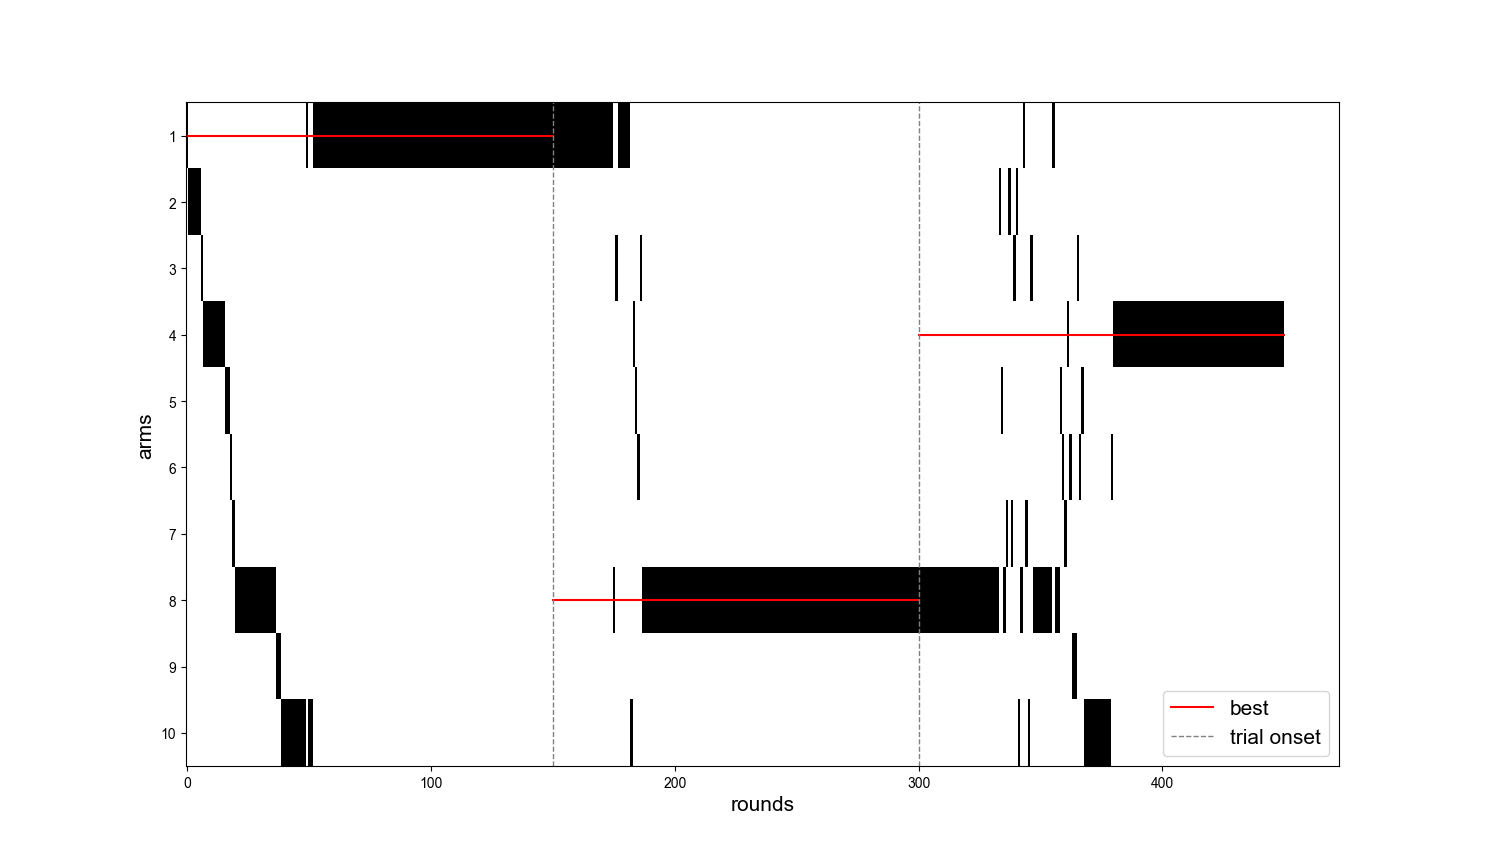
\includegraphics[width=0.9\textwidth]{figures/selections_1.png}
    \caption{\textsc{Selection evolution over rounds} - \textit{the x-axis represents the available arms, while the y-axis the number of rounds, with the dotted vertical lines indicating the start of a new trial with 150 rounds each. The model selections are the black vertical lines for an arm and a
    round. The red horizontal lines signal the arm with the highest reward probability, thus representing the best (and greediest) selection.}}
    \label{fig:sel1}
\end{figure}


\subsection{Learning}
Given a selected option, the environment (bandit) samples and returns a reward $R\in [0, 1]$.
Then, the connections $\textbf{W}^{MP}$ for the neuron corresponding to the option $k$ are updated according to the following plasticity rule:

\begin{equation}
    \Delta \textbf{W}^{MP}_{k} = \tilde{\eta}_{k} \left(R\cdot W^{+}- \textbf{W}^{MP}_{k}\right)
\end{equation}

\noindent
Where $W^{+}$ is a constant value that sets the upper bound for the synaptic weights, and it is set to $W^{+} = 5$, while $\tilde{\eta}_{k}$ is the learning rate for the option $k$ determined by a function of the current weights $\textbf{W}^{MP}_{k}$ and its shape is the same as $\Phi_{v}$, but with
different parameters.



